% =====================================================================
%  Σημασιολογικός Ιστός — 1η Εργασία (Θέμα 25):
%  Οντολογική μοντελοποίηση ταξιδιωτικού πρακτορείου και ερωτήματα SPARQL
%  Πρότυπο: IEEE Conference (IEEEtran)
%
%  ΟΔΗΓΙΕΣ OVERLEAF:
%    1. New Project -> Upload -> ανέβασε αυτό το αρχείο + τον φάκελο figures/
%    2. Menu -> Compiler: LuaLaTeX   (ΟΧΙ pdfLaTeX — χρειάζεται για τα ελληνικά)
%  Αν βγει σφάλμα γραμματοσειράς: άλλαξε το "STIX Two Text" σε "FreeSerif".
% =====================================================================
\documentclass[conference]{IEEEtran}

\usepackage{fontspec}
\setmainfont{STIX Two Text}            % Times-like, με ελληνικούς χαρακτήρες
\setsansfont{FreeSans}                 % sans serif με ελληνικά (ονόματα κλάσεων)
\setmonofont{FreeMono}                 % monospace με ελληνικά
\usepackage{polyglossia}
\setdefaultlanguage{greek}
\setotherlanguage{english}

\usepackage{amsmath,amssymb}
\usepackage{graphicx}
\usepackage{booktabs}
\usepackage{cite}
\usepackage{xcolor}
\usepackage{listings}
\usepackage{url}
\graphicspath{{figures/}}

\renewcommand{\IEEEkeywordsname}{Λέξεις-κλειδιά}

\lstdefinelanguage{SPARQL}{
  morekeywords={SELECT,DISTINCT,WHERE,FILTER,OPTIONAL,UNION,ORDER,BY,ASC,DESC,GROUP,
    HAVING,COUNT,SUM,AVG,MIN,BIND,AS,NOT,EXISTS,VALUES,PREFIX,a,GROUP_CONCAT,
    CONCAT,COALESCE,IF,BOUND,LANG,STR,STRAFTER,separator},
  sensitive=true, morestring=[b]", morecomment=[l]{\#}}
\lstset{language=SPARQL, basicstyle=\ttfamily\scriptsize, keywordstyle=\bfseries\color{blue!55!black},
  stringstyle=\color{red!50!black}, frame=single, framerule=0.3pt, rulecolor=\color{black!35},
  columns=fullflexible, keepspaces=true, showstringspaces=false, breaklines=true, xleftmargin=2pt, xrightmargin=2pt,
  aboveskip=4pt, belowskip=4pt}

\newcommand{\query}[1]{\par\medskip\noindent\textit{#1}\par\nobreak\smallskip}
\newcommand{\cls}[1]{\textsf{#1}}          % όνομα κλάσης
\newcommand{\prop}[1]{\textit{#1}}         % όνομα ιδιότητας
\newcommand{\ind}[1]{\texttt{#1}}          % όνομα στιγμιοτύπου

\begin{document}

\title{Οντολογική μοντελοποίηση ταξιδιωτικού πρακτορείου\\σε OWL~2 και ερωτήματα SPARQL}

\author{\IEEEauthorblockN{Απόστολος Δαγκλής}
\IEEEauthorblockA{Τμήμα Μηχανικών Πληροφορικής και Ηλεκτρονικών Συστημάτων\\
Διεθνές Πανεπιστήμιο της Ελλάδος (ΔΙΠΑΕ)\\
Α.Μ.: 2021031 \quad daglisapo1@gmail.com}}

\maketitle

% ---------------------------------------------------------------------
\begin{abstract}
Η εργασία παρουσιάζει μια οντολογία OWL~2 για τη δομή και τη λειτουργία ενός
ταξιδιωτικού πρακτορείου (θέμα~25). Η οντολογία περιγράφει προορισμούς και τη
γεωγραφική τους ιεραρχία, πακέτα διακοπών και τις υπηρεσίες που τα αποτελούν
(διαμονή, πτήσεις, ακτοπλοΐα, μεταφορές, οργανωμένες εκδρομές, ασφάλιση), πελάτες,
προσωπικό και υποκαταστήματα, κρατήσεις, πληρωμές, αξιολογήσεις και διαφημιστικές
καμπάνιες. Περιλαμβάνει 45 κλάσεις, 55 ιδιότητες (33 αντικειμένων και 22 δεδομένων)
και 117 στιγμιότυπα. Εκτός από την ιεραρχία, χρησιμοποιεί ξένες κλάσεις,
περιορισμούς πληθικότητας, ορισμένες κλάσεις με ικανές και αναγκαίες συνθήκες,
περιορισμούς τύπων δεδομένων, αντίστροφες, μεταβατικές και συμμετρικές ιδιότητες
και αλυσίδες ιδιοτήτων. Η συνέπεια ελέγχθηκε με τους reasoners HermiT και Pellet:
η οντολογία είναι συνεπής και δεν έχει unsatisfiable κλάσεις, ενώ τέσσερα σκόπιμα
λάθη μοντελοποίησης εντοπίστηκαν σωστά. Ο reasoner συνάγει 97 νέα γεγονότα, όπως
την κατάταξη πελατών και πακέτων σε ορισμένες κλάσεις και τις χώρες που επισκέπτεται
κάθε πακέτο. Τέλος, παρουσιάζονται 11 ερωτήματα SPARQL· τα τέσσερα από αυτά
επιστρέφουν αποτελέσματα μόνο αφού ληφθούν υπόψη τα συμπεράσματα του reasoner.
\end{abstract}

\begin{IEEEkeywords}
σημασιολογικός ιστός, οντολογία, OWL~2, Protégé, HermiT, Pellet, SPARQL, ταξιδιωτικό πρακτορείο
\end{IEEEkeywords}

% ---------------------------------------------------------------------
\section{Εισαγωγή}

Μια οντολογία είναι ρητή και τυπική περιγραφή των εννοιών ενός πεδίου, των σχέσεών
τους και των περιορισμών που ισχύουν μεταξύ τους~\cite{noy2001,antoniou}. Σε αντίθεση
με ένα σχήμα βάσης δεδομένων, μια οντολογία OWL~\cite{owl2primer} έχει τυπική
σημασιολογία βασισμένη σε περιγραφικές λογικές. Έτσι ένας reasoner μπορεί να ελέγξει
αν οι δηλώσεις είναι συνεπείς μεταξύ τους και να συναγάγει γνώση που δεν έχει
δηλωθεί ρητά. Τα δεδομένα αναζητούνται με τη γλώσσα SPARQL~\cite{sparql11}.

Στόχος της εργασίας είναι η σημασιολογική αναπαράσταση ενός ταξιδιωτικού
πρακτορείου: τι προσφέρει (πακέτα και υπηρεσίες), πού (προορισμοί), σε ποιους
(πελάτες), με ποιους (προσωπικό, συνεργάτες) και πώς το προβάλλει (καμπάνιες).
Δεν πρόκειται για σχεδιασμό πληροφοριακού συστήματος. Το ζητούμενο είναι η
οντολογία να «γνωρίζει» κανόνες του πεδίου, για παράδειγμα ότι ένα πακέτο με
πτήση είναι \cls{FlightPackage} ή ότι ένας πελάτης με τουλάχιστον 1000 πόντους
είναι VIP. Τα συμπεράσματα αυτά αξιοποιούνται στη συνέχεια στα ερωτήματα SPARQL.

Η ενότητα~II ορίζει το πεδίο και τα ερωτήματα επάρκειας, η~III τη μεθοδολογία
και τα εργαλεία, η~IV τον σχεδιασμό της οντολογίας και η~V τον έλεγχο με reasoner.
Η ενότητα~VI παρουσιάζει τα ερωτήματα SPARQL και η~VII τα συμπεράσματα.

% ---------------------------------------------------------------------
\section{Γνωστικό πεδίο και ερωτήματα επάρκειας}

Το πεδίο είναι ένα (φανταστικό) πρακτορείο, το \ind{Aegean Horizons Travel}, με
υποκαταστήματα σε Θεσσαλονίκη και Αθήνα. Το πρακτορείο συνθέτει πακέτα διακοπών
από υπηρεσίες τρίτων (ξενοδοχεία, αεροπορικές και ακτοπλοϊκές εταιρείες) και από
δικές του οργανωμένες εκδρομές με οδηγούς/συνοδούς. Οι πελάτες κάνουν κρατήσεις
μέσω ταξιδιωτικών συμβούλων, πληρώνουν με διάφορους τρόπους και αξιολογούν τα
πακέτα. Το τμήμα προβολής οργανώνει καμπάνιες σε διάφορα κανάλια.

Σύμφωνα με τη μεθοδολογία των Noy και McGuinness~\cite{noy2001}, το εύρος της
οντολογίας ορίστηκε από ερωτήματα επάρκειας (competency questions) που πρέπει να
μπορεί να απαντήσει:
\begin{enumerate}
\item Ποια πακέτα υπάρχουν, πού πηγαίνουν, πόσο κοστίζουν και τι περιλαμβάνουν;
\item Ποια πακέτα περιλαμβάνουν πτήση, νησιωτικό προορισμό ή συνοδό;
\item Πόσα έσοδα έφερε κάθε πακέτο και πώς το αξιολογούν οι πελάτες;
\item Ποιοι πελάτες είναι VIP και ποιοι σύμβουλοι τους εξυπηρέτησαν;
\item Ποιες κρατήσεις δεν έχουν εξοφληθεί;
\item Ποια πακέτα προβάλλονται χωρίς να έχουν πωλήσεις;
\item Ποιες χώρες και περιοχές καλύπτει το πρακτορείο;
\end{enumerate}
Αυτά τα ερωτήματα καθόρισαν και τι \emph{δεν} μοντελοποιήθηκε: για παράδειγμα,
θέσεις αεροσκαφών, τιμολόγηση ανά εποχή και λογιστική του πρακτορείου.

% ---------------------------------------------------------------------
\section{Μεθοδολογία και εργαλεία}

Ακολουθήθηκαν τα βήματα του~\cite{noy2001}: ορισμός πεδίου, απαρίθμηση όρων,
ιεραρχία κλάσεων (κυρίως από πάνω προς τα κάτω), ιδιότητες, περιορισμοί
(facets) και στιγμιότυπα. Η οντολογία γράφτηκε σε σύνταξη Turtle
(\path{travel_agency.ttl}) και μετατράπηκε σε RDF/XML (\path{travel_agency.owl}),
που ανοίγει απευθείας στο Protégé~\cite{protege}. Για τον έλεγχο χρησιμοποιήθηκαν
οι reasoners HermiT~\cite{hermit} και Pellet~\cite{pellet} μέσω της βιβλιοθήκης
owlready2~\cite{owlready} (Python), που περιλαμβάνει τους ίδιους reasoners με το
Protégé. Τα ερωτήματα SPARQL γράφτηκαν για την καρτέλα \emph{SPARQL Query} του
Protégé. Τα αποτελέσματα που παρουσιάζονται εδώ παράχθηκαν αυτόματα από τα ίδια
αρχεία με τη βιβλιοθήκη rdflib, ώστε να αναπαράγονται με μία εντολή. Τα
διαγράμματα δημιουργήθηκαν με Graphviz από τα triples της οντολογίας.

% ---------------------------------------------------------------------
\section{Σχεδιασμός της οντολογίας}

\subsection{Κλάσεις και ιεραρχία}

Η ιεραρχία (Σχ.~\ref{fig:classes}) έχει έξι ρίζες με υποκλάσεις και έξι
αυτόνομες κλάσεις. Οι ρίζες είναι ανά δύο ξένες μεταξύ τους με ένα αξίωμα
\texttt{AllDisjointClasses}, ώστε ένα στιγμιότυπο να μην μπορεί να είναι ταυτόχρονα
π.χ. πρόσωπο και τοποθεσία.

\begin{figure*}[!t]
\centering
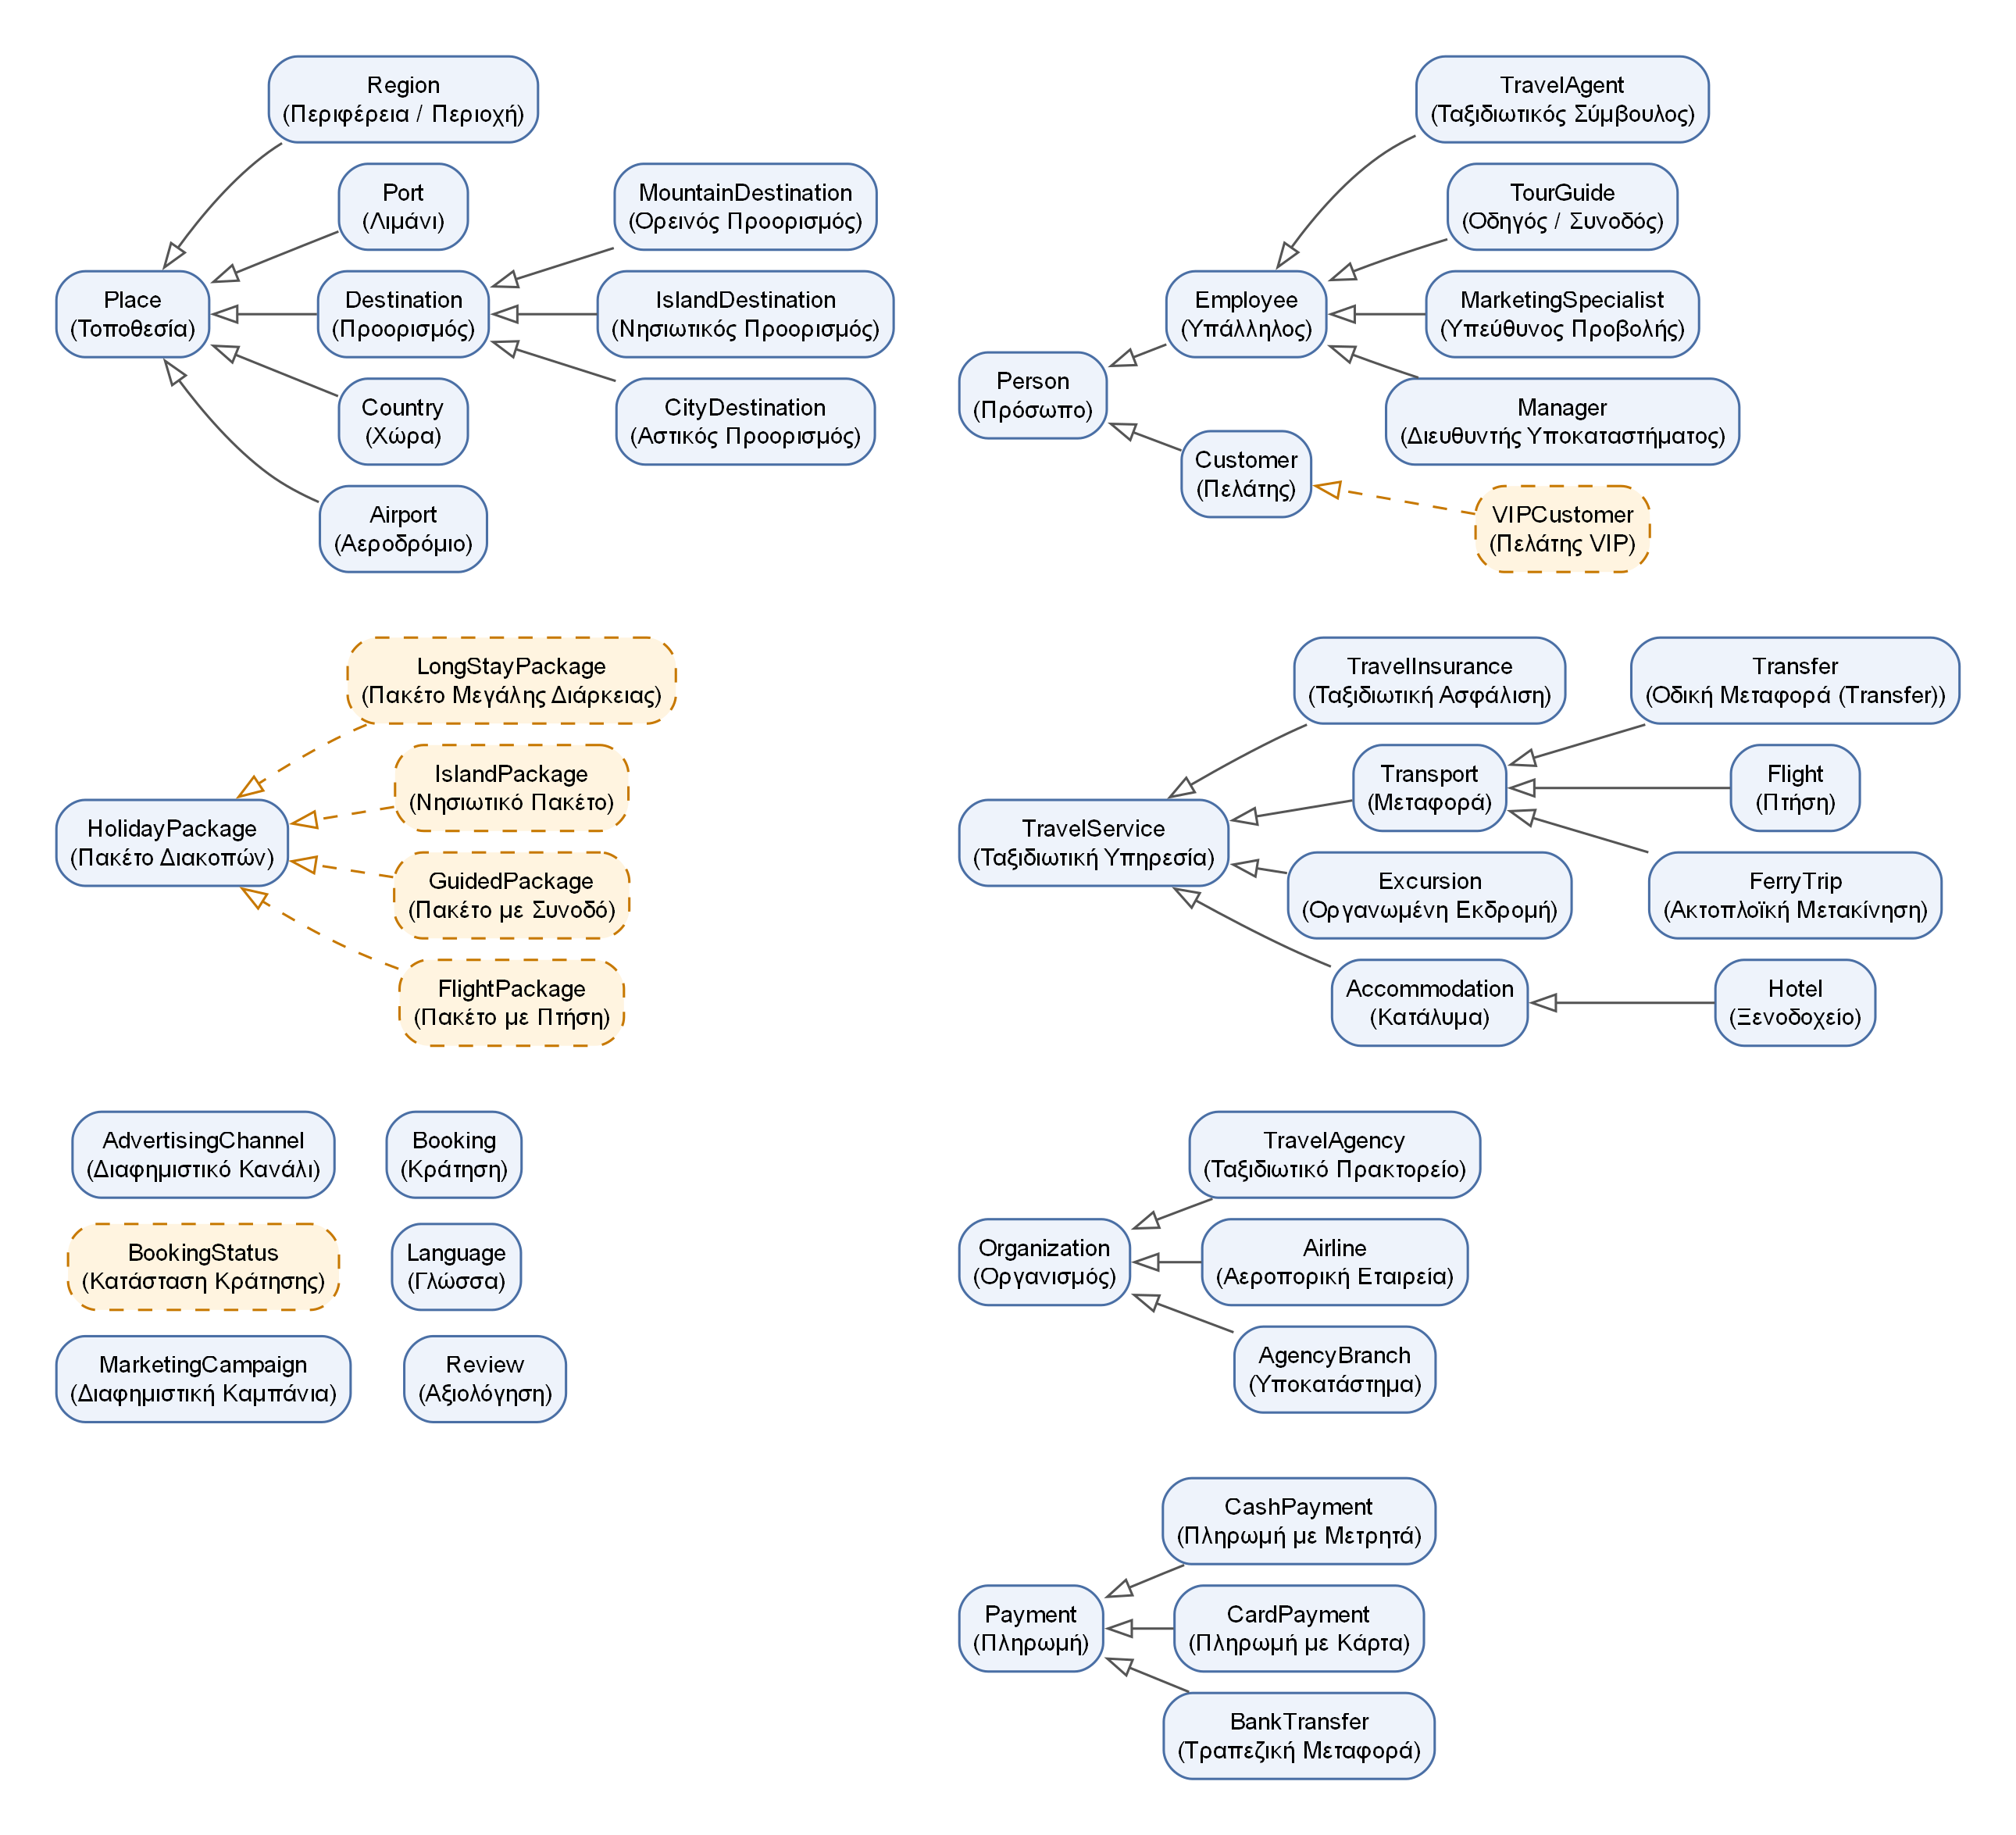
\includegraphics[width=0.92\textwidth]{class_hierarchy.png}
\caption{Ιεραρχία κλάσεων. Τα βέλη δείχνουν από την υποκλάση στην υπερκλάση. Με
διακεκομμένο περίγραμμα οι ορισμένες κλάσεις (owl:equivalentClass)· η υπερκλάση
τους (διακεκομμένο βέλος) δεν δηλώνεται, αλλά προκύπτει από τον ορισμό.}
\label{fig:classes}
\end{figure*}

\begin{itemize}
\item \cls{Person}: \cls{Customer} (με την ορισμένη υποκλάση \cls{VIPCustomer}) και
\cls{Employee} με υποκλάσεις \cls{TravelAgent}, \cls{TourGuide},
\cls{MarketingSpecialist} και \cls{Manager}. Οι τρεις πρώτες δηλώνονται ξένες. Ο
\cls{Manager} όχι, γιατί ένας διευθυντής υποκαταστήματος μπορεί να είναι και
σύμβουλος (π.χ. η \ind{MariaPapadopoulou}). Επίσης \cls{Customer} και
\cls{Employee} δεν είναι ξένες: ένας υπάλληλος μπορεί να αγοράσει πακέτο.
\item \cls{Organization}: \cls{TravelAgency}, \cls{AgencyBranch}, \cls{Airline}.
\item \cls{Place}: \cls{Country}, \cls{Region}, \cls{Destination} (με
\cls{CityDestination}, \cls{IslandDestination}, \cls{MountainDestination}),
\cls{Airport}, \cls{Port}.
\item \cls{TravelService}: οι υπηρεσίες από τις οποίες συντίθεται ένα πακέτο,
δηλαδή \cls{Accommodation}/\cls{Hotel}, \cls{Transport} (\cls{Flight},
\cls{FerryTrip}, \cls{Transfer}), \cls{Excursion} και \cls{TravelInsurance}.
\item \cls{HolidayPackage} με τέσσερις ορισμένες υποκλάσεις (\cls{FlightPackage},
\cls{IslandPackage}, \cls{GuidedPackage}, \cls{LongStayPackage}).
\item \cls{Payment}: \cls{CardPayment}, \cls{BankTransfer}, \cls{CashPayment} (ξένες).
\item Αυτόνομες: \cls{Booking}, \cls{BookingStatus}, \cls{Review},
\cls{MarketingCampaign}, \cls{AdvertisingChannel}, \cls{Language}.
\end{itemize}

Για κάθε υποκλάση ελέγχθηκε ότι ένα στιγμιότυπό της είναι πράγματι και στιγμιότυπο
της υπερκλάσης (π.χ. κάθε \cls{Hotel} είναι \cls{Accommodation}, κάθε
\cls{Flight} είναι \cls{Transport}) και ότι όλες οι ιδιότητες που κληρονομούνται
έχουν νόημα. Γι' αυτό το \cls{Airport} είναι \cls{Place} και όχι
\cls{Destination}: ένα αεροδρόμιο δεν είναι προορισμός διακοπών.

\subsection{Ιδιότητες αντικειμένων}

Ο Πίνακας~\ref{tab:objprops} δίνει τις 33 ιδιότητες αντικειμένων και το
Σχ.~\ref{fig:props} τις σχέσεις domain$\rightarrow$range. Επτά ζεύγη είναι
αντίστροφα (\prop{owl:inverseOf}), ώστε η σχέση να δηλώνεται μία φορά και να
διατρέχεται και από τις δύο πλευρές. Για παράδειγμα, στα δεδομένα δηλώνεται μόνο
το \prop{bookedBy}, και το \prop{hasBooking} του πελάτη προκύπτει.

\begin{table}[!t]
\caption{Ιδιότητες αντικειμένων (F: functional, IF: inverse functional,
T: transitive, S: symmetric, Irr: irreflexive)}
\label{tab:objprops}
\centering\scriptsize
\setlength{\tabcolsep}{3pt}
\resizebox{\columnwidth}{!}{%
\begin{tabular}{@{}lll@{}}
\toprule
Ιδιότητα & Domain $\rightarrow$ Range & Σημειώσεις \\
\midrule
bookedBy / hasBooking & Booking $\rightarrow$ Customer & F / IF, αντίστροφες \\
forPackage & Booking $\rightarrow$ HolidayPackage & F \\
handledBy & Booking $\rightarrow$ TravelAgent & \\
hasPayment & Booking $\rightarrow$ Payment & IF \\
hasStatus & Booking $\rightarrow$ BookingStatus & F \\
servedBy & Customer $\rightarrow$ TravelAgent & αλυσίδα \\
travelsWith & Customer $\rightarrow$ Customer & S, Irr \\
includesService & HolidayPackage $\rightarrow$ TravelService & \\
hasDestination & HolidayPackage $\rightarrow$ Destination & $\sqsubseteq$ visitsPlace \\
visitsPlace & HolidayPackage $\rightarrow$ Place & αλυσίδα \\
offeredBy / offersPackage & HolidayPackage $\rightarrow$ TravelAgency & αντίστροφες \\
locatedIn & -- $\rightarrow$ Place & T \\
departsFrom, arrivesAt & Transport $\rightarrow$ Place & \\
operatedBy & Flight $\rightarrow$ Airline & \\
hasGuide / guides & -- $\rightarrow$ TourGuide & αντίστροφες \\
visitsDestination & Excursion $\rightarrow$ Destination & \\
worksFor / employs & Employee $\rightarrow$ AgencyBranch & αντίστροφες \\
manages & Manager $\rightarrow$ AgencyBranch & IF, $\sqsubseteq$ worksFor \\
branchOf / hasBranch & AgencyBranch $\rightarrow$ TravelAgency & F, αντίστροφες \\
speaksLanguage & Person $\rightarrow$ Language & \\
writtenBy / writesReview & Review $\rightarrow$ Customer & F, αντίστροφες \\
reviews & Review $\rightarrow$ HolidayPackage & F \\
promotes / promotedBy & MarketingCampaign $\rightarrow$ HolidayPackage & αντίστροφες \\
usesChannel & MarketingCampaign $\rightarrow$ AdvertisingChannel & \\
createdBy & MarketingCampaign $\rightarrow$ MarketingSpecialist & \\
\bottomrule
\end{tabular}}
\end{table}

Ορισμένες επιλογές χρειάζονται εξήγηση:
\begin{itemize}
\item Το \prop{locatedIn} είναι \emph{μεταβατικό} και δεν έχει domain. Χρησιμοποιείται
για τοποθεσίες (Οία $\rightarrow$ Σαντορίνη $\rightarrow$ Κυκλάδες $\rightarrow$
Ελλάδα), αλλά και για ξενοδοχεία και υποκαταστήματα. Αν οριζόταν domain
\cls{Place}, κάθε ξενοδοχείο θα κατατασσόταν ως τοποθεσία, και επειδή
\cls{TravelService} και \cls{Place} είναι ξένες, η οντολογία θα γινόταν ασυνεπής.
\item Το \prop{visitsPlace} ορίζεται με την αλυσίδα
$\mathit{hasDestination}\circ\mathit{locatedIn}\sqsubseteq\mathit{visitsPlace}$ και
έχει υπο-ιδιότητα το \prop{hasDestination}. Έτσι ένα πακέτο «επισκέπτεται» τον
προορισμό του και κάθε περιοχή και χώρα που τον περιέχει, χωρίς να δηλωθούν.
\item Το \prop{servedBy} ορίζεται με την αλυσίδα
$\mathit{hasBooking}\circ\mathit{handledBy}\sqsubseteq\mathit{servedBy}$: ο πελάτης
εξυπηρετήθηκε από κάθε σύμβουλο που διεκπεραίωσε κάποια κράτησή του.
\item Το \prop{manages} είναι υπο-ιδιότητα του \prop{worksFor}, οπότε για τους
διευθυντές δεν χρειάζεται να δηλωθεί και ότι εργάζονται στο υποκατάστημα.
\end{itemize}

\begin{figure}[!t]
\centering
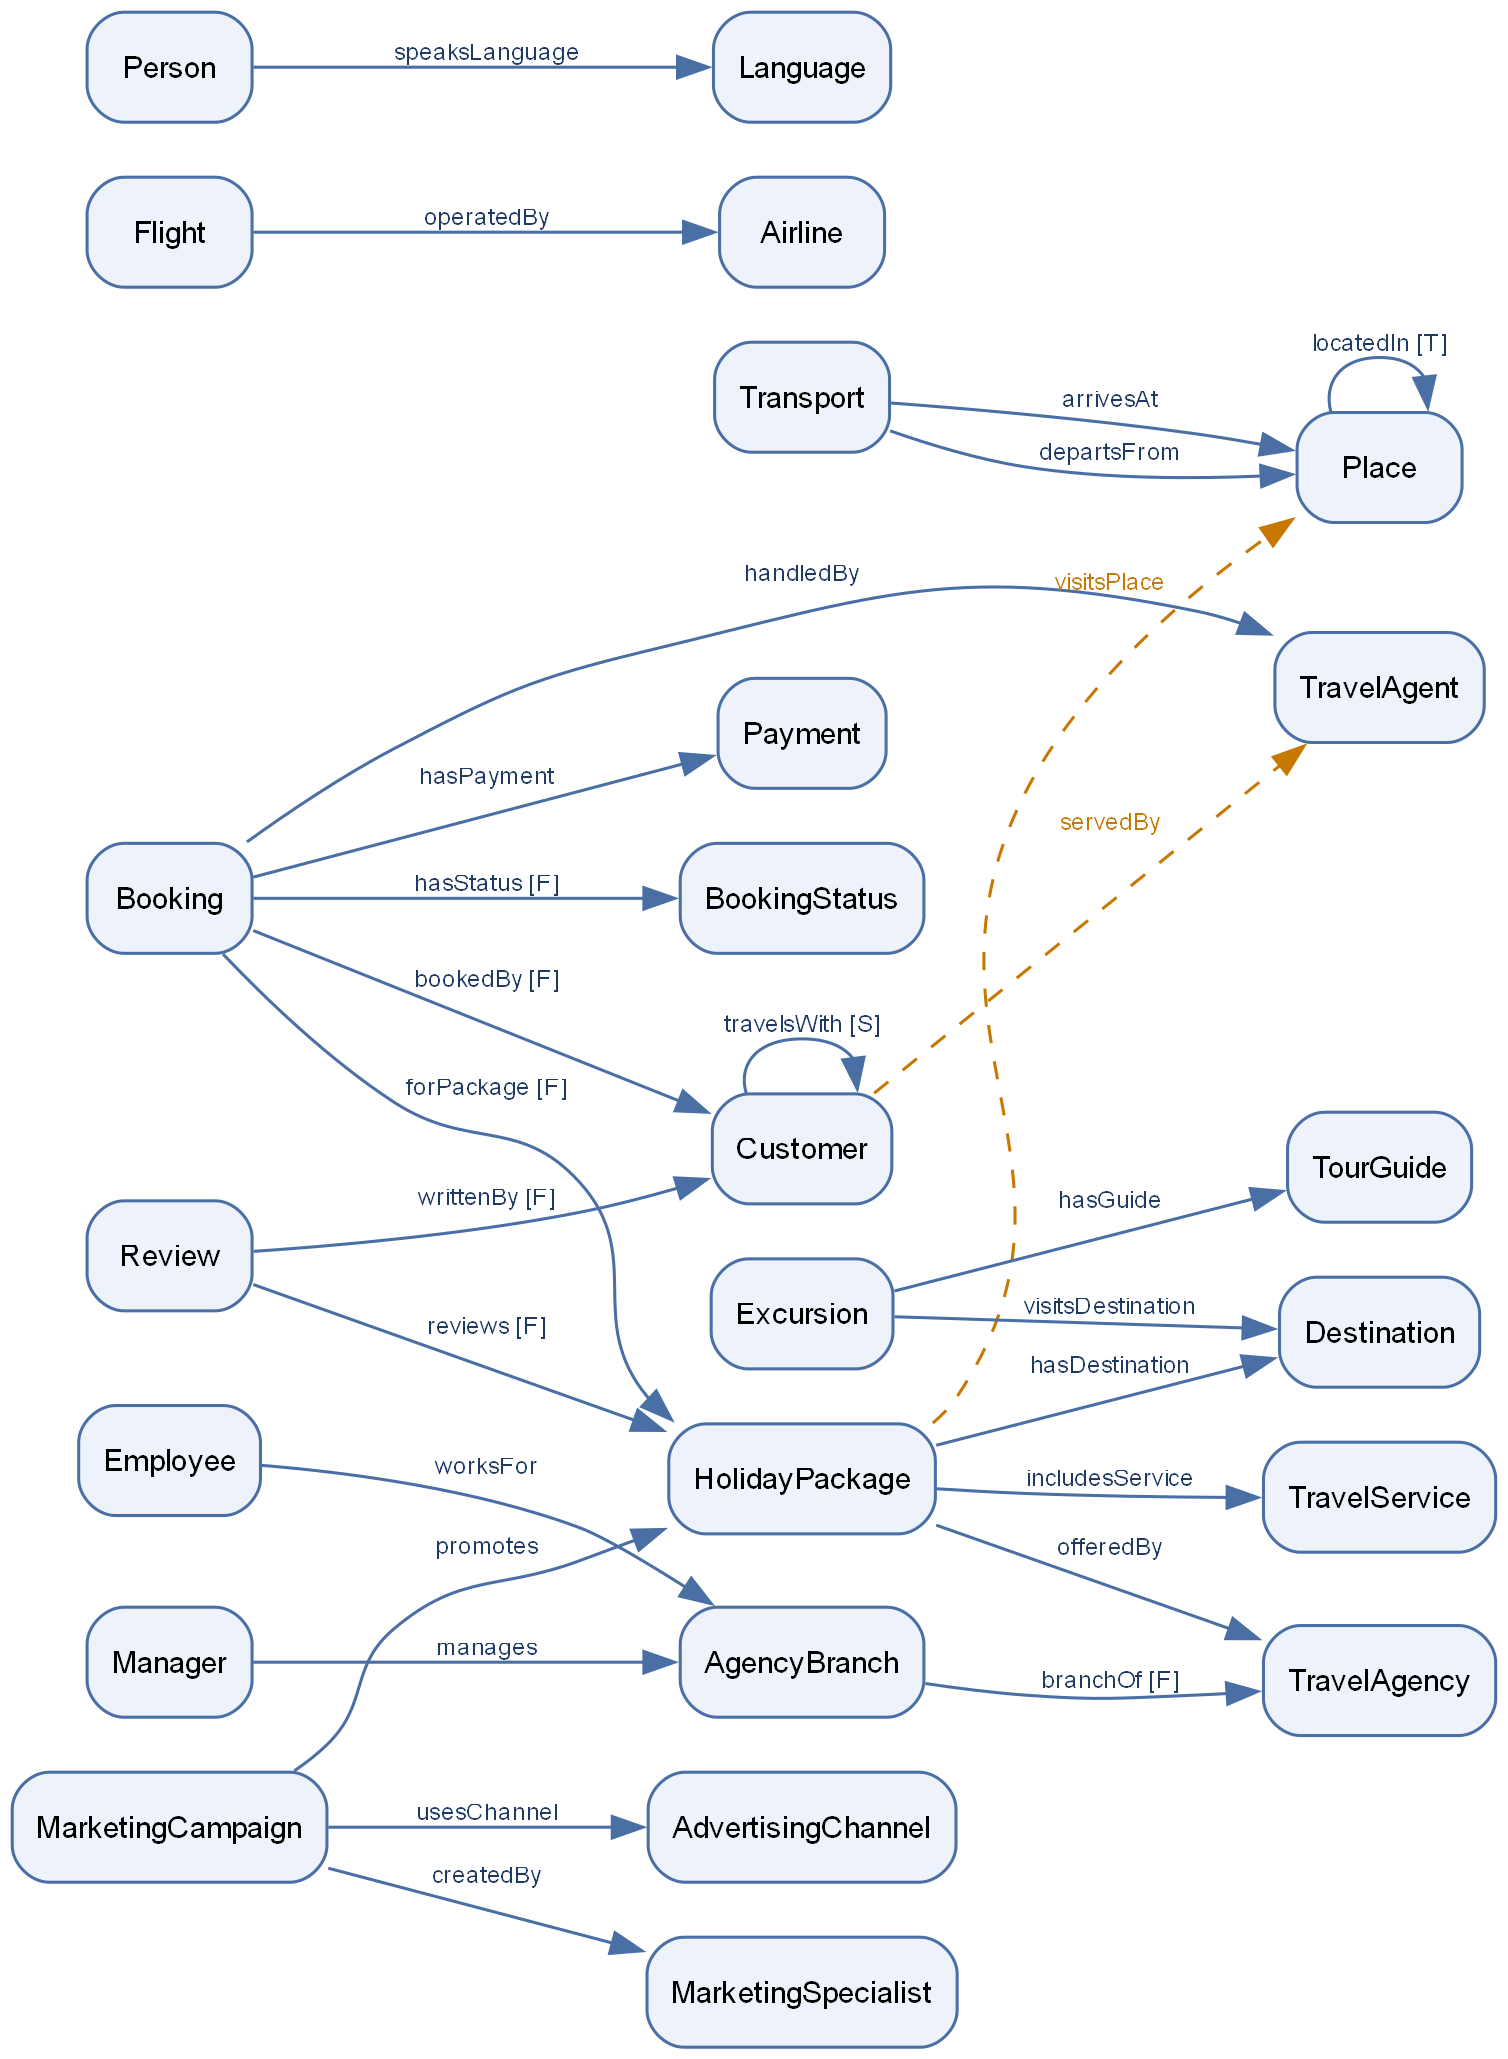
\includegraphics[width=\columnwidth]{object_properties.png}
\caption{Ιδιότητες αντικειμένων ως ακμές domain$\rightarrow$range. Από κάθε ζεύγος
αντίστροφων εμφανίζεται μόνο η μία. Διακεκομμένες οι ιδιότητες που ορίζονται με
αλυσίδα. [F] functional, [T] transitive, [S] symmetric.}
\label{fig:props}
\end{figure}

\subsection{Ιδιότητες δεδομένων}

Οι 22 ιδιότητες δεδομένων είναι: \prop{name}, \prop{firstName}, \prop{lastName},
\prop{email}, \prop{loyaltyPoints}, \prop{salary}, \prop{hireDate},
\prop{pricePerPerson}, \prop{durationDays}, \prop{departureDate},
\prop{bookingDate}, \prop{numberOfTravellers}, \prop{amount}, \prop{rating},
\prop{reviewText}, \prop{starRating}, \prop{flightNumber}, \prop{iataCode},
\prop{maxParticipants}, \prop{budget}, \prop{startDate} και \prop{endDate}. Οι
περισσότερες είναι functional. Οι τύποι είναι \texttt{xsd:string},
\texttt{xsd:integer}, \texttt{xsd:positiveInteger}, \texttt{xsd:decimal} και
\texttt{xsd:dateTime}. Το \texttt{xsd:date} δεν χρησιμοποιήθηκε επειδή δεν ανήκει
στο OWL~2 datatype map και οι reasoners δεν το υποστηρίζουν. Το range της
\prop{rating} είναι ο περιορισμένος τύπος \texttt{xsd:integer[1..5]}.

\subsection{Αξιώματα και περιορισμοί}

Εκτός από τα domain/range και τα χαρακτηριστικά των ιδιοτήτων, η οντολογία
περιέχει τα εξής αξιώματα (σε σύνταξη περιγραφικής λογικής):

\noindent\textit{Αναγκαίες συνθήκες (subclass axioms):}
{\footnotesize
\begin{align*}
\mathit{Booking} \sqsubseteq\ & {=}1\,\mathit{bookedBy}.\mathit{Customer}\\
 \sqcap\ & {=}1\,\mathit{forPackage}.\mathit{HolidayPackage}\\
 \sqcap\ & {=}1\,\mathit{hasStatus}.\mathit{BookingStatus}\\
\mathit{HolidayPackage} \sqsubseteq\ & \exists\mathit{hasDestination}.\mathit{Destination}\\
 \sqcap\ & \exists\mathit{includesService}.\mathit{Accommodation}\\
 \sqcap\ & {=}1\,\mathit{pricePerPerson}.\mathit{decimal}\\
\mathit{Flight} \sqsubseteq\ & {=}1\,\mathit{departsFrom}.\mathit{Airport}\\
 \sqcap\ & {=}1\,\mathit{arrivesAt}.\mathit{Airport}\\
 \sqcap\ & {=}1\,\mathit{operatedBy}.\mathit{Airline}\\
\mathit{Excursion} \sqsubseteq\ & \exists\mathit{hasGuide}.\mathit{TourGuide}\\
 \sqcap\ & \exists\mathit{visitsDestination}.\mathit{Destination}\\
\mathit{Employee} \sqsubseteq\ & \exists\mathit{worksFor}.\mathit{AgencyBranch}\\
\mathit{Hotel} \sqsubseteq\ & \exists\mathit{starRating}.\mathit{integer}[1..5]
\end{align*}}
Παρόμοιοι περιορισμοί υπάρχουν για τα \cls{AgencyBranch}, \cls{FerryTrip},
\cls{Accommodation}, \cls{TourGuide}, \cls{Manager}, \cls{Payment}, \cls{Review} και
\cls{MarketingCampaign}.

\noindent\textit{Ικανές και αναγκαίες συνθήκες (ορισμένες κλάσεις):}
{\footnotesize
\begin{align*}
\mathit{VIPCustomer} \equiv\ & \mathit{Customer}\\
 \sqcap\ & \exists\mathit{loyaltyPoints}.\mathit{integer}[\geq 1000]\\
\mathit{FlightPackage} \equiv\ & \mathit{HolidayPackage}\\
 \sqcap\ & \exists\mathit{includesService}.\mathit{Flight}\\
\mathit{IslandPackage} \equiv\ & \mathit{HolidayPackage}\\
 \sqcap\ & \exists\mathit{hasDestination}.\mathit{IslandDestination}\\
\mathit{GuidedPackage} \equiv\ & \mathit{HolidayPackage}\\
 \sqcap\ & \exists\mathit{includesService}.(\exists\mathit{hasGuide}.\mathit{TourGuide})\\
\mathit{LongStayPackage} \equiv\ & \mathit{HolidayPackage}\\
 \sqcap\ & \exists\mathit{durationDays}.\mathit{integer}[\geq 7]\\
\mathit{BookingStatus} \equiv\ & \{\mathit{Confirmed}, \mathit{Pending}, \mathit{Cancelled}\}
\end{align*}}

Σε κανένα στιγμιότυπο δεν δηλώνεται ρητά κάποια από τις πέντε πρώτες κλάσεις.
Η συμμετοχή τους προκύπτει από τον reasoner. Ο ορισμός του \cls{GuidedPackage}
συνδυάζεται με το αξίωμα του \cls{Excursion}: η ξενάγηση στο Λούβρο δεν έχει
ακόμη δηλωμένο συνοδό, αλλά η οντολογία γνωρίζει ότι κάθε εκδρομή έχει έναν.
Επομένως το \ind{ParisCityBreak} κατατάσσεται ως πακέτο με συνοδό. Η κλάση
\cls{BookingStatus} είναι απαριθμητή (\texttt{owl:oneOf}) και οι τιμές της, μαζί με
τις γλώσσες και τα διαφημιστικά κανάλια, δηλώνονται διαφορετικές μεταξύ τους
(\texttt{owl:AllDifferent}). Χωρίς αυτή τη δήλωση, λόγω της απουσίας Unique Name
Assumption στην OWL, ο reasoner δεν θα μπορούσε να αποκλείσει ότι π.χ. το
\ind{Confirmed} και το \ind{Cancelled} είναι το ίδιο άτομο.

\subsection{Στιγμιότυπα}

Τα 117 στιγμιότυπα περιλαμβάνουν: 1 πρακτορείο, 2 υποκαταστήματα, 7 υπαλλήλους,
9 πελάτες, 3 χώρες, 6 περιοχές, 7 προορισμούς, 5 αεροδρόμια, 2 λιμάνια,
2 αεροπορικές εταιρείες, 6 πτήσεις, 1 ακτοπλοϊκή διαδρομή, 2 transfers,
6 ξενοδοχεία, 5 εκδρομές, 2 ασφάλειες, 7 πακέτα, 12 κρατήσεις, 9 πληρωμές,
8 αξιολογήσεις, 3 καμπάνιες, 5 κανάλια, 4 γλώσσες και 3 καταστάσεις κράτησης.
Ενδεικτικά, το πακέτο \ind{SantoriniEscape} (Σχ.~\ref{fig:instances}) έχει
προορισμό τη Σαντορίνη, διάρκεια 7 ημερών, τιμή 890\,€ ανά άτομο, και
περιλαμβάνει τις πτήσεις HA101/HA102 Θεσσαλονίκη--Σαντορίνη, transfer, το
ξενοδοχείο \ind{CalderaViewHotel} (5 αστέρων), την κρουαζιέρα στο ηφαίστειο με
συνοδό τη Σοφία Αλεξίου και βασική ασφάλιση. Ο πελάτης \ind{DimitrisKarras} (1850
πόντοι) το έκλεισε για δύο άτομα μέσω του συμβούλου \ind{NikosGeorgiou} και
πλήρωσε 1780\,€ με κάρτα.

\begin{figure*}[!t]
\centering
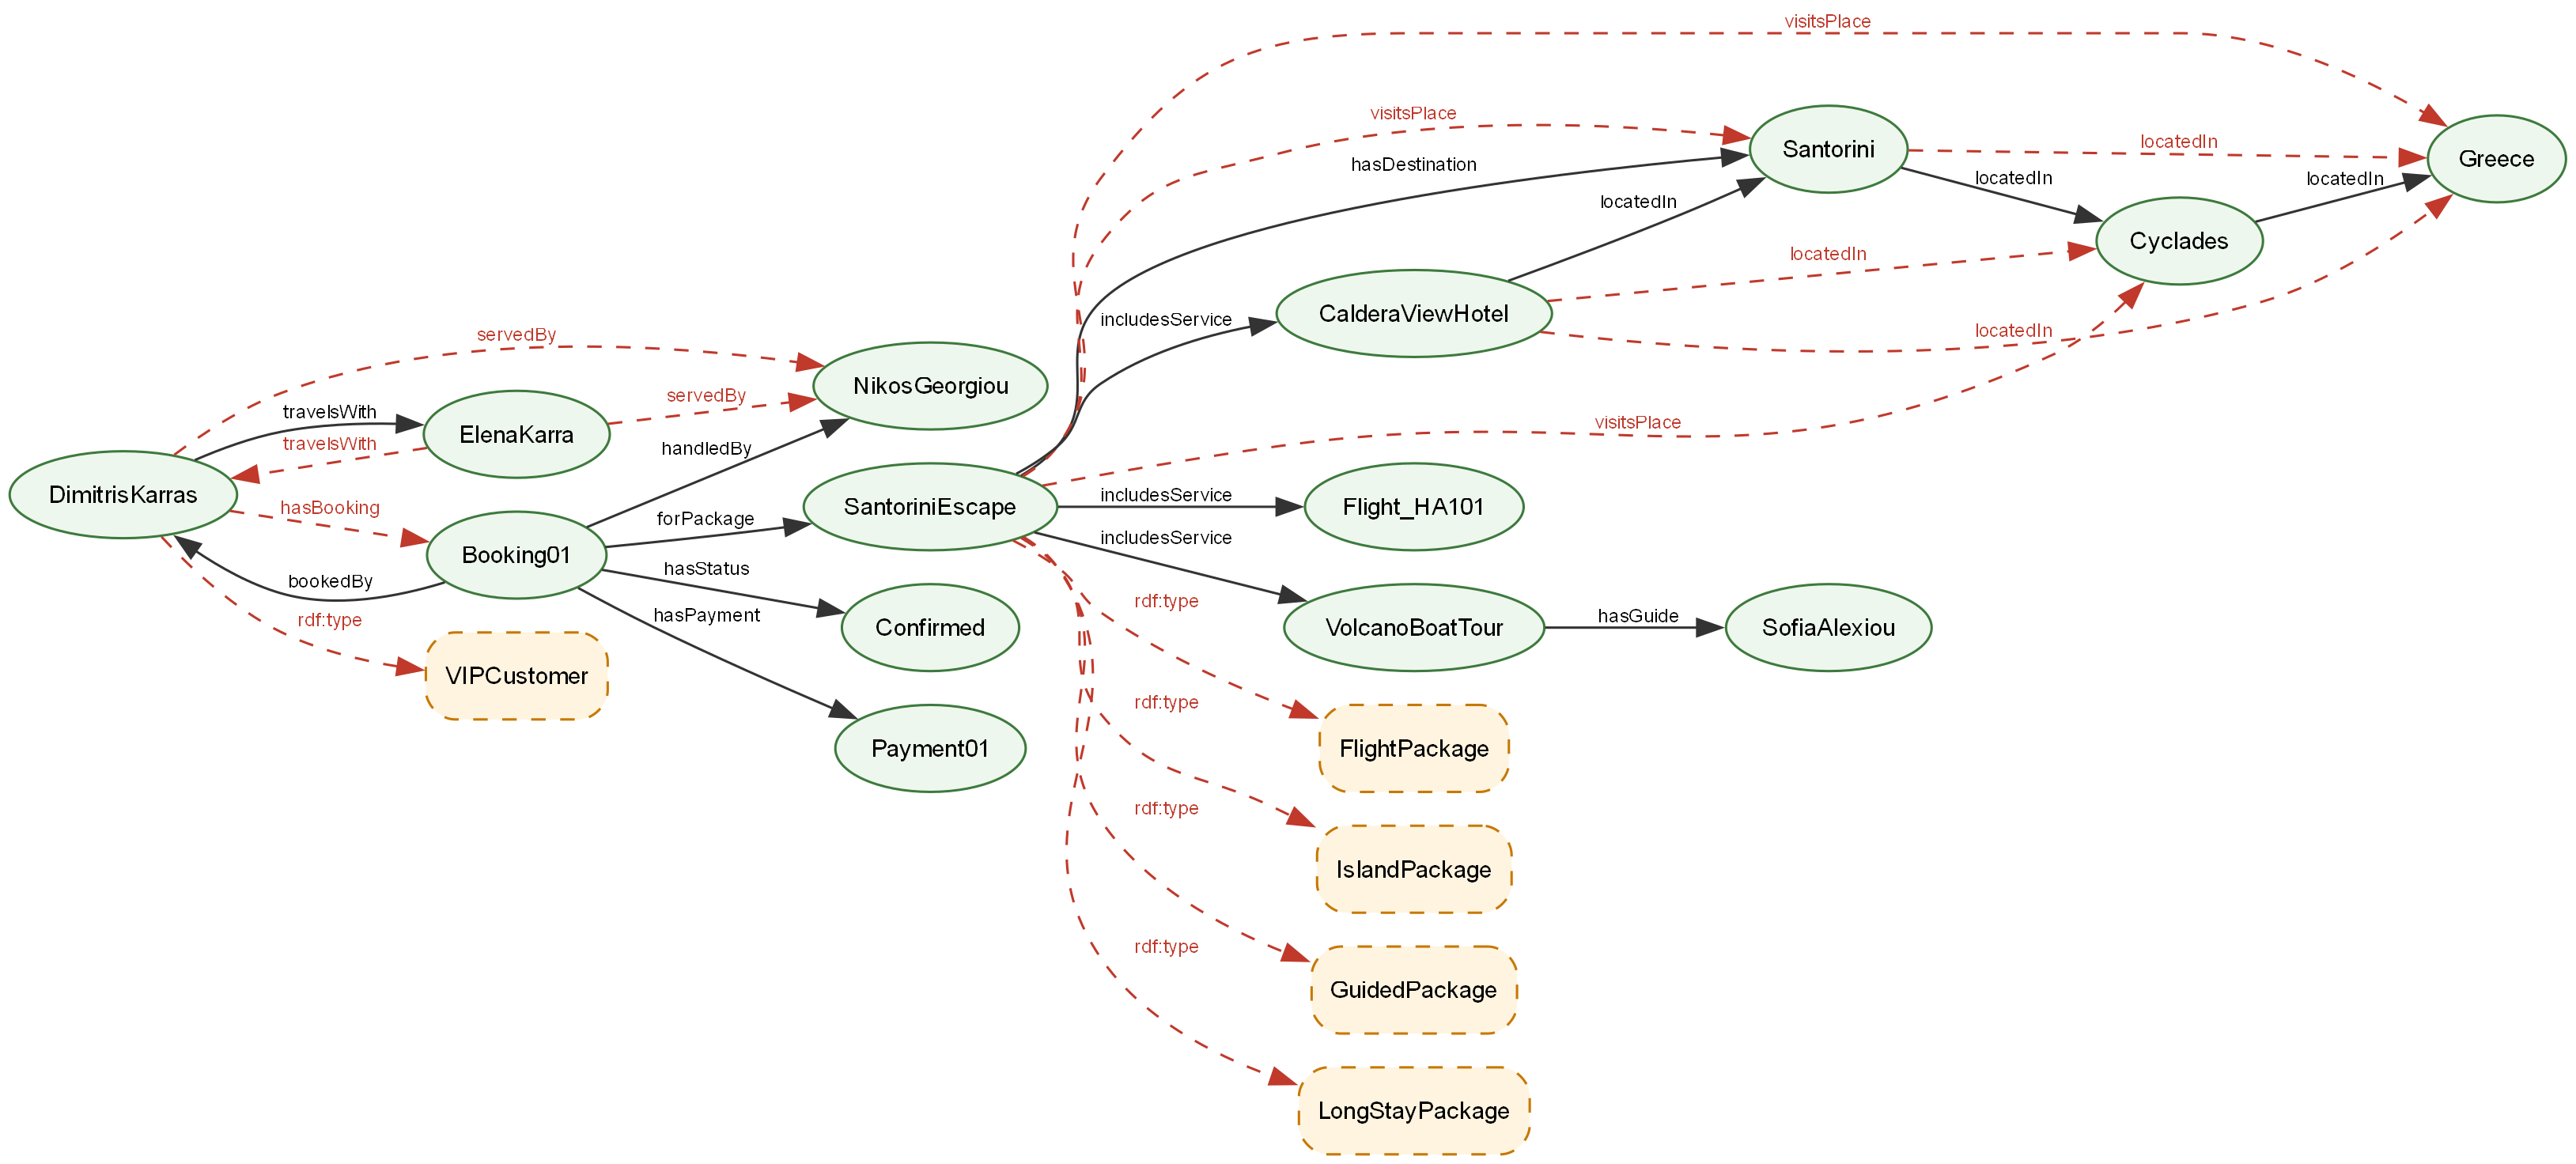
\includegraphics[width=0.9\textwidth]{instance_graph.png}
\caption{Απόσπασμα στιγμιοτύπων γύρω από την κράτηση \ind{Booking01}. Συνεχείς
ακμές: ρητές δηλώσεις. Κόκκινες διακεκομμένες: γεγονότα που συνάγει ο reasoner
(Pellet) από τους ορισμούς κλάσεων, τις αντίστροφες, τη συμμετρική και τη
μεταβατική ιδιότητα και τις αλυσίδες ιδιοτήτων.}
\label{fig:instances}
\end{figure*}

\subsection{Εναλλακτικές που εξετάστηκαν}

\begin{itemize}
\item \emph{Ξενοδοχείο ως οργανισμός.} Αρχικά εξετάστηκε το \cls{Hotel} να είναι
και \cls{Organization}, ως συνεργαζόμενη επιχείρηση. Επειδή όμως το ξενοδοχείο
μπαίνει στα πακέτα ως υπηρεσία διαμονής, και οι \cls{Organization} και
\cls{TravelService} είναι ξένες, η κλάση γίνεται unsatisfiable
(Ενότητα~\ref{sec:negative}). Κρατήθηκε μόνο ως υπηρεσία.
\item \emph{Κατηγορίες πακέτων ως ρητές υποκλάσεις.} Θα ήταν πιο απλό να δηλώνεται
χειροκίνητα ότι ένα πακέτο είναι νησιωτικό ή με πτήση. Αυτό όμως επαναλαμβάνει
πληροφορία που ήδη υπάρχει στα δεδομένα και μπορεί να γίνει ασυνεπές όταν
αλλάξει το πακέτο. Οι ορισμένες κλάσεις αφήνουν την κατάταξη στον reasoner.
\item \emph{Κατάσταση κράτησης ως string.} Απορρίφθηκε υπέρ μιας απαριθμητής κλάσης,
ώστε να μην υπάρχουν τιμές εκτός λίστας και να είναι δυνατή η σύνδεση με ετικέτες.
\item \emph{Ελάχιστη πληθικότητα για «συχνό πελάτη»} (π.χ. $\geq 3$ κρατήσεις).
Απορρίφθηκε: λόγω της υπόθεσης ανοιχτού κόσμου (OWA) και της απουσίας UNA, ο
reasoner δεν μετρά στιγμιότυπα όπως μια βάση δεδομένων. Θα χρειαζόταν δήλωση
\texttt{AllDifferent} για όλες τις κρατήσεις. Ο VIP πελάτης ορίστηκε με βάση τους
πόντους.
\item \emph{Τιμές ανά εποχή και διαθεσιμότητα θέσεων.} Αφορούν περισσότερο τη
λειτουργία ενός συστήματος κρατήσεων παρά τη σημασιολογία του πεδίου και θα
αύξαναν πολύ την πολυπλοκότητα. Η τιμή μοντελοποιήθηκε ως μία τιμή ανά άτομο.
\end{itemize}

% ---------------------------------------------------------------------
\section{Έλεγχος με reasoner}

\subsection{Συνέπεια και συμπερασμός}

Η οντολογία ελέγχθηκε με τους HermiT και Pellet~2.3.1. Και οι δύο την έκριναν
\emph{συνεπή} (consistent), χωρίς \emph{unsatisfiable} κλάσεις, σε περίπου 3\,s
ο καθένας. Τα συμπεράσματα συνοψίζονται στον Πίνακα~\ref{tab:inferred}.

\begin{table}[!t]
\caption{Γεγονότα που συνάγει ο reasoner (Pellet)}
\label{tab:inferred}
\centering\scriptsize
\setlength{\tabcolsep}{3pt}
\begin{tabular}{@{}lrl@{}}
\toprule
Συμπέρασμα & Πλήθος & Αιτία \\
\midrule
VIPCustomer & 4 & ορισμός (πόντοι $\geq 1000$) \\
FlightPackage & 4 & ορισμός \\
GuidedPackage & 5 & ορισμός + αξίωμα Excursion \\
IslandPackage & 3 & ορισμός \\
LongStayPackage & 2 & ορισμός (διάρκεια $\geq 7$) \\
locatedIn & 36 & μεταβατικότητα \\
visitsPlace & 22 & υπο-ιδιότητα + αλυσίδα \\
servedBy & 12 & αλυσίδα hasBooking$\circ$handledBy \\
worksFor / employs & 2 / 2 & manages $\sqsubseteq$ worksFor, inverse \\
subClassOf & 5 & υπερκλάση των ορισμένων κλάσεων \\
\midrule
Σύνολο & 97 & \\
\bottomrule
\end{tabular}
\end{table}

Οι τιμές των αντίστροφων και των συμμετρικών ιδιοτήτων (π.χ. 12 τιμές
\prop{hasBooking} από το \prop{bookedBy}, η \prop{travelsWith} προς την αντίθετη
κατεύθυνση) δεν μετρώνται στον πίνακα, γιατί το owlready2 τις παρέχει ήδη πριν από
τον reasoner. Τα αποτελέσματα των δύο reasoners συμπίπτουν, με μία εξαίρεση: οι 8
τιμές \prop{visitsPlace} που προκύπτουν απευθείας από την υπο-ιδιότητα
\prop{hasDestination} (π.χ. \ind{SantoriniEscape} \prop{visitsPlace}
\ind{Santorini}) εμφανίζονται μόνο στην έξοδο του Pellet, όπως την επιστρέφει το
owlready2. Η οντολογία μαζί με τα συμπεράσματα αποθηκεύτηκε στο
\path{travel_agency_inferred.owl}. Στο Protégé το ίδιο αποτέλεσμα προκύπτει με
\emph{Reasoner $\rightarrow$ Start reasoner} και \emph{File $\rightarrow$ Export
inferred axioms as ontology}.

\subsection{Σκόπιμα λάθη}
\label{sec:negative}

Για να επιβεβαιωθεί ότι τα αξιώματα πράγματι περιορίζουν τα μοντέλα, σε αντίγραφα
της οντολογίας προστέθηκαν τέσσερα λάθη (Πίνακας~\ref{tab:negative}). Ο HermiT τα
εντόπισε όλα. Στο Α εξετάστηκε επίσης η οντολογία χωρίς στιγμιότυπα, όπου η
\cls{Hotel} εμφανίζεται ως unsatisfiable. Στα Β--Δ τα αξιώματα κλάσεων είναι
ικανοποιήσιμα και η ασυνέπεια οφείλεται μόνο στα δεδομένα. Το Δ δείχνει την
απουσία UNA: η κράτηση με δύο πελάτες δεν απορρίπτεται επειδή «οι πελάτες είναι
δύο», αλλά επειδή η ταύτισή τους, που επιβάλλει η functional \prop{bookedBy}, θα
έδινε στο ίδιο άτομο δύο τιμές στη functional \prop{loyaltyPoints}.

\begin{table}[!t]
\caption{Σκόπιμα λάθη και αποτέλεσμα του HermiT}
\label{tab:negative}
\centering\scriptsize
\setlength{\tabcolsep}{3pt}
\begin{tabular}{@{}p{0.47\columnwidth}p{0.45\columnwidth}@{}}
\toprule
Λάθος & Αποτέλεσμα \\
\midrule
Α. Hotel $\sqsubseteq$ Organization & ασυνεπής· Hotel unsatisfiable (Hotel $\sqsubseteq$ TravelService, ξένη με Organization) \\
Β. Review01 rating 7 & ασυνεπής (range integer[1..5]) \\
Γ. LouvreTour hasGuide NikosGeorgiou & ασυνεπής (range TourGuide, ξένη με TravelAgent) \\
Δ. Booking01 bookedBy KaterinaLazarou & ασυνεπής (functional bookedBy και loyaltyPoints) \\
\bottomrule
\end{tabular}
\end{table}

% ---------------------------------------------------------------------
\section{Ερωτήματα SPARQL}

Υλοποιήθηκαν 11 ερωτήματα (αρχεία \path{queries/q01}--\path{q11}). Όλα
χρησιμοποιούν το πρόθεμα\\
\texttt{\footnotesize PREFIX ta: <http://www.semanticweb.org/dagklis/}\\
\texttt{\footnotesize \ \ ontologies/2026/travel-agency\#>}\\
και, όπου χρειάζεται, το \texttt{rdfs:}. Τα Q1--Q7 εκτελούνται στην
\path{travel_agency.owl}. Τα Q8--Q11 βασίζονται σε συμπεράσματα του reasoner και
εκτελούνται στην \path{travel_agency_inferred.owl}: στην asserted οντολογία
επιστρέφουν 0 γραμμές (το Q10 επιστρέφει τα 7 πακέτα χωρίς καμία κατηγορία).
Χρησιμοποιείται το inferred αρχείο ώστε τα αποτελέσματα να μην εξαρτώνται από
το αν το plugin SPARQL του Protégé λαμβάνει υπόψη τον reasoner.

\query{Q1 -- Κατάλογος πακέτων (ORDER BY)}
Όλα τα πακέτα με προορισμό, διάρκεια και τιμή, από το φθηνότερο.
\begin{lstlisting}
SELECT ?package ?destination ?days ?price
WHERE {
  ?p a ta:HolidayPackage ; ta:name ?package ;
     ta:hasDestination ?d ; ta:durationDays ?days ;
     ta:pricePerPerson ?price .
  ?d ta:name ?destination .
} ORDER BY ASC(?price) ?destination
\end{lstlisting}
Επιστρέφει 8 γραμμές, από το Thessaloniki Gastronomy Weekend (230\,€, 2 ημέρες)
έως το Cyclades Island Hopping (1450\,€, 10 ημέρες). Το τελευταίο εμφανίζεται δύο
φορές, μία για κάθε προορισμό του (Σαντορίνη, Μύκονος).

\query{Q2 -- Πακέτα με πτήση κάτω από 1000\,€ (FILTER, OPTIONAL)}
Για κάθε πτήση δίνεται η αεροπορική εταιρεία μέσω του property path
\texttt{ta:operatedBy/ta:name}, και προαιρετικά η εκδρομή και ο συνοδός της.
\begin{lstlisting}
SELECT ?package ?price ?flight ?airline ?excursion ?guide
WHERE {
  ?p a ta:HolidayPackage ; ta:name ?package ;
     ta:pricePerPerson ?price ; ta:includesService ?f .
  ?f a ta:Flight ; ta:flightNumber ?flight ;
     ta:operatedBy/ta:name ?airline .
  FILTER (?price < 1000)
  OPTIONAL {
    ?p ta:includesService ?e .
    ?e a ta:Excursion ; ta:name ?excursion .
    OPTIONAL { ?e ta:hasGuide ?g .
      ?g ta:firstName ?gf ; ta:lastName ?gl .
      BIND (CONCAT(?gf, " ", ?gl) AS ?guide) }
  }
} ORDER BY ?price ?flight
\end{lstlisting}
\begin{center}\scriptsize\setlength{\tabcolsep}{3pt}
\begin{tabular}{@{}lrlll@{}}
\toprule
package & price & flight & airline & guide \\
\midrule
Paris City Break & 560 & MS440 & MedSky & -- \\
Roman Holiday & 720 & MS330 & MedSky & Γ. Νικολάου \\
Roman Holiday & 720 & MS331 & MedSky & Γ. Νικολάου \\
Santorini Escape & 890 & HA101 & HellasAir & Σ. Αλεξίου \\
Santorini Escape & 890 & HA102 & HellasAir & Σ. Αλεξίου \\
\bottomrule
\end{tabular}\end{center}
(Η στήλη excursion παραλείπεται για λόγους χώρου.) Στο Paris City Break το
εσωτερικό OPTIONAL μένει κενό, γιατί η ξενάγηση στο Λούβρο δεν έχει δηλωμένο
συνοδό. Το Cyclades Island Hopping αποκλείεται από το FILTER.

\query{Q3 -- Έσοδα ανά πακέτο (COUNT, SUM, GROUP BY)}
Μόνο επιβεβαιωμένες κρατήσεις, ταξινόμηση κατά έσοδα.
\begin{lstlisting}
SELECT ?package (COUNT(?b) AS ?bookings)
       (SUM(?n) AS ?travellers) (SUM(?amount) AS ?revenue)
WHERE {
  ?b a ta:Booking ; ta:forPackage ?p ;
     ta:hasStatus ta:Confirmed ;
     ta:numberOfTravellers ?n ;
     ta:hasPayment/ta:amount ?amount .
  ?p ta:name ?package .
} GROUP BY ?package ORDER BY DESC(?revenue)
\end{lstlisting}
\begin{center}\scriptsize\setlength{\tabcolsep}{4pt}
\begin{tabular}{@{}lrrr@{}}
\toprule
package & bookings & travellers & revenue \\
\midrule
Cyclades Island Hopping & 1 & 2 & 2900 \\
Mykonos Summer & 2 & 4 & 2560 \\
Roman Holiday & 2 & 3 & 2160 \\
Arachova Winter Weekend & 2 & 6 & 1860 \\
Santorini Escape & 1 & 2 & 1780 \\
Thessaloniki Gastronomy Weekend & 1 & 2 & 460 \\
\bottomrule
\end{tabular}\end{center}
Το Paris City Break λείπει: η μόνη κράτησή του είναι σε αναμονή.

\query{Q4 -- Καλύτερα αξιολογημένα πακέτα (AVG, HAVING)}
\begin{lstlisting}
SELECT ?package (COUNT(?r) AS ?reviews)
       (AVG(?rating) AS ?avgRating)
       (MIN(?rating) AS ?worst)
WHERE {
  ?r a ta:Review ; ta:reviews ?p ; ta:rating ?rating .
  ?p ta:name ?package .
} GROUP BY ?package
  HAVING (AVG(?rating) >= 4)
  ORDER BY DESC(?avgRating) ?package
\end{lstlisting}
Επιστρέφει 4 πακέτα: Cyclades Island Hopping, Santorini Escape και Thessaloniki
Gastronomy Weekend με μέσο όρο 5, και Arachova Winter Weekend με 4. Τα Mykonos
Summer και Roman Holiday (μέσος όρος 3,5 από δύο αξιολογήσεις το καθένα)
αποκλείονται από το HAVING.

\query{Q5 -- Επαφές πελάτη με το προσωπικό (UNION)}
Οι σύμβουλοι που διεκπεραίωσαν τις κρατήσεις του Πέτρου Μιχαήλ, μαζί με τους
συνοδούς των εκδρομών που περιλαμβάνονται στα πακέτα του.
\begin{lstlisting}
SELECT DISTINCT ?role ?employee ?context
WHERE {
  ?b ta:bookedBy ta:PetrosMichail ; ta:forPackage ?p .
  ?p ta:name ?pname .
  { ?b ta:handledBy ?e .
    BIND ("Ταξιδιωτικός σύμβουλος" AS ?role) }
  UNION
  { ?p ta:includesService ?x .
    ?x a ta:Excursion ; ta:hasGuide ?e ; ta:name ?xname .
    BIND ("Οδηγός / Συνοδός" AS ?role) }
  ?e ta:firstName ?f ; ta:lastName ?l .
  BIND (CONCAT(?f, " ", ?l) AS ?employee)
  BIND (IF(BOUND(?xname),
           CONCAT(?pname, ": ", ?xname), ?pname)
        AS ?context)
} ORDER BY ?role ?employee
\end{lstlisting}
Αποτέλεσμα: ο συνοδός Γιώργος Νικολάου (Roman Holiday: Ξενάγηση στα Μουσεία του
Βατικανού) και οι σύμβουλοι Μαρία Παπαδοπούλου (Cyclades Island Hopping) και Νίκος
Γεωργίου (Roman Holiday). Το \texttt{?context} υπολογίζεται μετά το UNION, γιατί
η μεταβλητή \texttt{?pname} δεν είναι ορατή μέσα στα σκέλη του.

\query{Q6 -- Προβολή χωρίς πωλήσεις (FILTER NOT EXISTS)}
\begin{lstlisting}
SELECT ?package ?campaign ?budget
       (GROUP_CONCAT(?channel; separator=", ")
          AS ?channels)
WHERE {
  ?p a ta:HolidayPackage ; ta:name ?package .
  FILTER NOT EXISTS { ?b ta:forPackage ?p ;
                         ta:hasStatus ta:Confirmed . }
  ?c a ta:MarketingCampaign ; ta:promotes ?p ;
     ta:name ?campaign ; ta:budget ?budget ;
     ta:usesChannel/ta:name ?channel .
} GROUP BY ?package ?campaign ?budget
\end{lstlisting}
Επιστρέφει μία γραμμή: το Paris City Break προβάλλεται από την καμπάνια «City
breaks στην Ευρώπη» (3500\,€, κανάλια: social media και ραδιοφωνικό σποτ) χωρίς
καμία επιβεβαιωμένη κράτηση.

\query{Q7 -- Υπόλοιπα κρατήσεων (BIND, COALESCE)}
\begin{lstlisting}
SELECT ?booking ?customer ?package ?status
       ?cost ?paid ?balance
WHERE {
  ?b a ta:Booking ; ta:bookedBy ?c ; ta:forPackage ?p ;
     ta:numberOfTravellers ?n ; ta:hasStatus ?s .
  FILTER (?s != ta:Cancelled)
  ?s rdfs:label ?status . FILTER (LANG(?status) = "el")
  ?c ta:lastName ?customer .
  ?p ta:name ?package ; ta:pricePerPerson ?price .
  OPTIONAL { ?b ta:hasPayment/ta:amount ?amount . }
  BIND (?price * ?n AS ?cost)
  BIND (COALESCE(?amount, 0) AS ?paid)
  BIND (?cost - ?paid AS ?balance)
  BIND (STRAFTER(STR(?b), "#") AS ?booking)
} ORDER BY DESC(?balance) ?booking
\end{lstlisting}
Επιστρέφει τις 11 μη ακυρωμένες κρατήσεις. Οι δύο που είναι σε αναμονή έχουν
ανεξόφλητο υπόλοιπο: Booking10 (Καρρά, Santorini Escape, 890\,€) και Booking06
(Σταύρου, Paris City Break, 560\,€). Στις υπόλοιπες 9 το ποσό πληρωμής ισούται με
το κόστος (υπόλοιπο 0), κάτι που λειτουργεί και ως έλεγχος ορθότητας των δεδομένων.

\query{Q8 -- [Reasoning] Πελάτες VIP και σύμβουλοί τους}
\begin{lstlisting}
SELECT ?customer ?points
  (GROUP_CONCAT(DISTINCT ?agent; separator=", ")
     AS ?servedBy)
WHERE {
  ?c a ta:VIPCustomer ; ta:firstName ?f ; ta:lastName ?l ;
     ta:loyaltyPoints ?points .
  BIND (CONCAT(?f, " ", ?l) AS ?customer)
  OPTIONAL { ?c ta:servedBy/ta:lastName ?agent . }
} GROUP BY ?customer ?points ORDER BY DESC(?points)
\end{lstlisting}
\begin{center}\scriptsize\setlength{\tabcolsep}{4pt}
\begin{tabular}{@{}lrl@{}}
\toprule
customer & points & servedBy \\
\midrule
Πέτρος Μιχαήλ & 2600 & Γεωργίου, Παπαδοπούλου \\
Δημήτρης Καρράς & 1850 & Γεωργίου, Δημητρίου \\
Μάρθα Κώστα & 1200 & Γεωργίου, Δημητρίου \\
John Smith & 1000 & Γεωργίου \\
\bottomrule
\end{tabular}\end{center}
Εδώ χρησιμοποιούνται τρία είδη συμπερασμού: η κατάταξη στο \cls{VIPCustomer}, η
τιμή \prop{hasBooking} ως αντίστροφη του \prop{bookedBy}, και η αλυσίδα που ορίζει
το \prop{servedBy}. Ο John Smith (ακριβώς 1000 πόντοι) περιλαμβάνεται λόγω του
\texttt{minInclusive}, ενώ η Ιωάννα Σταύρου (999) όχι.

\query{Q9 -- [Reasoning] Πακέτα ανά χώρα}
\begin{lstlisting}
SELECT ?country (COUNT(DISTINCT ?p) AS ?packages)
  (GROUP_CONCAT(DISTINCT ?package; separator=", ")
     AS ?packageNames)
WHERE {
  ?p ta:visitsPlace ?c ; ta:name ?package .
  ?c a ta:Country ; ta:name ?country .
} GROUP BY ?country ORDER BY DESC(?packages) ?country
\end{lstlisting}
Αποτέλεσμα: Ελλάδα 5 πακέτα, Γαλλία 1 και Ιταλία 1. Κανένα πακέτο δεν συνδέεται
ρητά με χώρα. Η σύνδεση προκύπτει από την αλυσίδα του \prop{visitsPlace} σε
συνδυασμό με τη μεταβατικότητα του \prop{locatedIn} (π.χ. Σαντορίνη $\rightarrow$
Κυκλάδες $\rightarrow$ Ελλάδα).

\query{Q10 -- [Reasoning] Συναγόμενες κατηγορίες πακέτων (VALUES)}
\begin{lstlisting}
SELECT ?package
  (GROUP_CONCAT(?category; separator=", ")
     AS ?categories)
WHERE {
  ?p a ta:HolidayPackage ; ta:name ?package .
  OPTIONAL {
    VALUES ?class { ta:FlightPackage ta:IslandPackage
                    ta:GuidedPackage ta:LongStayPackage }
    ?p a ?class . ?class rdfs:label ?category .
    FILTER (LANG(?category) = "el")
  }
} GROUP BY ?package ORDER BY ?package
\end{lstlisting}
\begin{center}\scriptsize\setlength{\tabcolsep}{4pt}
\begin{tabular}{@{}ll@{}}
\toprule
package & categories \\
\midrule
Arachova Winter Weekend & -- \\
Cyclades Island Hopping & Πτήση, Νησιωτικό, Μεγάλης Διάρκειας \\
Mykonos Summer & Νησιωτικό, Με Συνοδό \\
Paris City Break & Πτήση, Με Συνοδό \\
Roman Holiday & Πτήση, Με Συνοδό \\
Santorini Escape & Πτήση, Νησιωτικό, Με Συνοδό, Μεγάλης Διάρκειας \\
Thessaloniki Gastr.\ Weekend & Με Συνοδό \\
\bottomrule
\end{tabular}\end{center}
(Οι ετικέτες εμφανίζονται συντομευμένες.) Το Arachova Winter Weekend δεν ανήκει
σε καμία κατηγορία: η μεταφορά του γίνεται οδικά, ο προορισμός είναι ορεινός, η
διάρκεια είναι 3 ημέρες και δεν περιλαμβάνει εκδρομή.

\query{Q11 -- [Reasoning] Ξενοδοχεία στην Ελλάδα (transitive)}
\begin{lstlisting}
SELECT ?hotel ?stars ?destination
WHERE {
  ?h a ta:Hotel ; ta:name ?hotel ; ta:starRating ?stars ;
     ta:locatedIn ta:Greece ; ta:locatedIn ?d .
  ?d a/rdfs:subClassOf* ta:Destination ;
     ta:name ?destination .
} ORDER BY DESC(?stars) ?hotel
\end{lstlisting}
Επιστρέφει τα 4 ελληνικά ξενοδοχεία: Caldera View Hotel (5$\star$, Σαντορίνη),
Mykonos Blue Suites (4$\star$, Μύκονος), Parnassos Chalet (4$\star$, Αράχωβα) και
White Tower Hotel (3$\star$, Θεσσαλονίκη). Το \texttt{a/rdfs:subClassOf*}
χρειάζεται γιατί ο reasoner αποθηκεύει μόνο τον πιο ειδικό τύπο κάθε στιγμιότυπου
(π.χ. \cls{IslandDestination}). Χωρίς reasoner, ίδιο αποτέλεσμα δίνει το property
path \texttt{ta:locatedIn+}. Η οντολογία όμως εκφράζει τη μεταβατικότητα ως ιδιότητα
της σχέσης, ώστε να ισχύει για κάθε ερώτημα χωρίς να την επαναλαμβάνει ο χρήστης.

% ---------------------------------------------------------------------
\section{Συμπεράσματα}

Η οντολογία καλύπτει τις βασικές έννοιες ενός ταξιδιωτικού πρακτορείου και
ξεπερνά το ενδεικτικό μέγεθος της εκφώνησης (45 κλάσεις, 55 ιδιότητες,
117 στιγμιότυπα). Ο έλεγχος με δύο reasoners έδειξε ότι είναι συνεπής. Τα τέσσερα
σκόπιμα λάθη έδειξαν ότι οι περιορισμοί πράγματι αποκλείουν λανθασμένα δεδομένα,
όπως βαθμολογία εκτός κλίμακας ή υπάλληλο σε λάθος ρόλο. Τα ερωτήματα SPARQL
απαντούν στα ερωτήματα επάρκειας της Ενότητας~II. Τα Q8--Q11 δείχνουν το κύριο
πλεονέκτημα έναντι μιας βάσης δεδομένων: πληροφορία όπως οι κατηγορίες πακέτων ή οι
χώρες που επισκέπτεται ένα πακέτο προκύπτει από κανόνες του πεδίου που
δηλώνονται μία φορά στην οντολογία.

Η οντολογία έχει και περιορισμούς. Λόγω OWA, η απουσία πληροφορίας δεν σημαίνει
άρνηση (π.χ. ένα πακέτο χωρίς δηλωμένη πτήση δεν συνάγεται ότι «δεν έχει πτήση»).
Γι' αυτό ερωτήματα όπως το Q6 χρησιμοποιούν τη SPARQL για άρνηση. Επίσης,
αριθμητικοί κανόνες μεταξύ ιδιοτήτων (π.χ. ότι το ποσό πληρωμής ισούται με τιμή
$\times$ ταξιδιώτες) δεν εκφράζονται σε OWL~2 DL. Εδώ ελέγχονται με SPARQL (Q7) και θα
μπορούσαν να εκφραστούν με SWRL ή SHACL. Επέκταση της εργασίας θα ήταν η
σύνδεση των προορισμών με το DBpedia/GeoNames (Linked Data), ώστε τα γεωγραφικά
στοιχεία να μη δηλώνονται τοπικά.

% ---------------------------------------------------------------------
\begin{thebibliography}{9}
\bibitem{noy2001} N.~F. Noy and D.~L. McGuinness, ``Ontology Development 101: A Guide
to Creating Your First Ontology,'' Stanford KSL Technical Report KSL-01-05, 2001.
\bibitem{antoniou} G.~Antoniou, P.~Groth, F.~van Harmelen, and R.~Hoekstra,
\textit{A Semantic Web Primer}, 3rd ed. Cambridge, MA: MIT Press, 2012.
\bibitem{owl2primer} W3C OWL Working Group, ``OWL 2 Web Ontology Language Primer
(Second Edition),'' W3C Recommendation, Dec. 2012.
\bibitem{sparql11} S.~Harris and A.~Seaborne (eds.), ``SPARQL 1.1 Query Language,''
W3C Recommendation, Mar. 2013.
\bibitem{protege} M.~A. Musen, ``The Protégé project: A look back and a look
forward,'' \textit{AI Matters}, vol.~1, no.~4, pp.~4--12, 2015.
\bibitem{hermit} B.~Glimm, I.~Horrocks, B.~Motik, G.~Stoilos, and Z.~Wang, ``HermiT:
An OWL 2 reasoner,'' \textit{J. Automated Reasoning}, vol.~53, no.~3,
pp.~245--269, 2014.
\bibitem{pellet} E.~Sirin, B.~Parsia, B.~Cuenca Grau, A.~Kalyanpur, and Y.~Katz,
``Pellet: A practical OWL-DL reasoner,'' \textit{J. Web Semantics}, vol.~5, no.~2,
pp.~51--53, 2007.
\bibitem{owlready} J.-B. Lamy, ``Owlready: Ontology-oriented programming in Python
with automatic classification and high level constructs for biomedical
ontologies,'' \textit{Artificial Intelligence in Medicine}, vol.~80, pp.~11--28, 2017.
\end{thebibliography}

\end{document}
